%%%%%%%%%%%%%%%%%%%%%%%%%%%%%%%%%%%%%%%%%%%%%%%%%%%%%%%%%%%%%%%%%%%%%%%%%%%%%%%
\section{Bias Between Continuous Energy and Multi-Group Calculations}
\label{sec:bias}
%%%%%%%%%%%%%%%%%%%%%%%%%%%%%%%%%%%%%%%%%%%%%%%%%%%%%%%%%%%%%%%%%%%%%%%%%%%%%%%

first paragraph:
-this will come from chapter 5 of my thesis


%%%%%%%%%%%%%%%%%%%%%%%%%%%%%%%%%%%%%%%%%%%%%%%%%%%%%%%%%%%%%%%%%%%%%%%%%%%%%%%
\section{Eigenvalue Bias}
\label{sec:bias-eigenvalues}

first paragraph: what are we comparing??
-reference eigenvalues from MC simulations
-reference MC simulation used to collapse MGXS
-multi-group MOC use MGXS to calculate an eigenvalue
-MG eigenvalue is compared to MC eigenvalue with Eqn.~\ref{eqn:delta-rho}

second paragraph: presented tabulated results
-Tab.~\ref{tab:keff-reference} - reference eigenvalues from OpenMC
  -difference between aniso and iso-in-lab: 65 pcm
-Tab.~\ref{tab:keff-bias-aniso} - OpenMC eigenvalues w/ MGXS generated from anisotropic OpenMC simulations
-Tab.~\ref{tab:keff-bias-iso-in-lab} - OpenMOC eigenvalues w/ MGXS generated from iso-in-lab OpenMC simulations

third paragraph: analyze results
-bias grows more negative with more energy groups
  -goes against intuition: eigenvalues should be more accurate w/ more groups
  -with enough groups (e.g., ultra-fine), MG and MC eigenvalues should match exactly
  -but with coarser group structures, the eigenvalues do not match
    -even with ``perfect'' group condensation with the ``true'' flux

\begin{equation}
\label{eqn:delta-rho}
\Delta\rho = \left(k_{eff}^{OpenMOC} - k_{eff}^{OpenMC}\right) \times 10^{5}
\end{equation}

-data is for 2D fuel pin with MGXS tallied by FSR

\begin{table}[h!]
  \centering
  \caption{Reference OpenMC eigenvalues for a 2D fuel pin.}
  \label{tab:keff-reference} 
  \begin{tabular}{c c}
  \toprule
  {\bf Anisotropic} &
  {\bf Isotropic in Lab} \\
  \midrule
  1.17486 $\pm$ 0.00001 & 1.17421 $\pm$ 0.00001 \\
  \bottomrule
\end{tabular}
\end{table}

\begin{table}[h!]
  \centering
  \caption{The eigenvalue bias with transport-corrected MGXS.}
  \label{tab:keff-bias-aniso} 
  \begin{tabular}{c S[table-format=6.1] S[table-format=6.1] S[table-format=6.1]}
  \toprule
  & \multicolumn{3}{c}{{\bf FSR Discretization}} \\
  \midrule
  \multicolumn{1}{c}{{\bf \# Groups}} &
  {\bf 1$\times$} & {\bf 4$\times$} & {\bf 16$\times$} \\
  \midrule
1 & 53 & 75 & 72 \\
2 & 37 & 1 & 4 \\
4 & -58 & -92 & -109 \\
8 & -74 & -145 & -170 \\
16 & -67 & -154 & -183 \\
25 & -124 & -221 & -245 \\
40 & -130 & -238 & -265 \\
70 & -131 & -281 & -274 \\
  \bottomrule
\end{tabular}
\end{table}

\begin{table}[h!]
  \centering
  \caption{The eigenvalue bias with isotropic-in-lab scattering.}
  \label{tab:keff-bias-iso-in-lab} 
  \begin{tabular}{c S[table-format=6.1] S[table-format=6.1] S[table-format=6.1]}
  \toprule
  & \multicolumn{3}{c}{{\bf FSR Discretization}} \\
  \midrule
  \multicolumn{1}{c}{{\bf \# Groups}} &
  {\bf 1$\times$} & {\bf 4$\times$} & {\bf 16$\times$} \\
  \midrule
1 & 80 & 55 & 66 \\
2 & 141 & 29 & 34 \\
4 & 27 & -43 & -57 \\
8 & 26 & -85 & -102 \\
16 & 35 & -91 & -111 \\
25 & -31 & -158 & -182 \\
40 & -38 & -174 & -202 \\
70 & -39 & -182 & -211 \\
  \bottomrule
\end{tabular}
\end{table}


%%%%%%%%%%%%%%%%%%%%%%%%%%%%%%%%%%%%%%%%%%%%%%%%%%%%%%%%%%%%%%%%%%%%%%%%%%%%%%%
\section{Multi-Group Flux Bias}
\label{sec:bias-flux}

first paragraph: present figures
-Fig.~\ref{fig:rel-err-energy} compares MG and MC flux by energy group
  -innermost and outermost rings of the fuel pin, and average across all rings
-Fig.~\ref{fig:rel-err-space} compares MG and MC flux by spatial zone
  -for three energy group ``ranges'' across all radial rings in the fuel pin
-describe the three energy ranges
  -range A: group for the U-238 capture resonance at 6.67 eV
  -range B: groups spanning the three lowest-lying U-238 capture resonances
  -range C: all U-238 resonance energy groups
  
second paragraph: analyze figures
-take analysis from my thesis
-the errors are largest for range A which most tightly encompasses a single resonance
-errors vary widely across fuel pin
-tie this into an argument of why this:
  (1) causes an eigenvalue bias
  (2) results from loss of angular information with scalar flux-weighted MGXS
-segue into next section on possible solutions

\begin{figure}[h!]
\centering
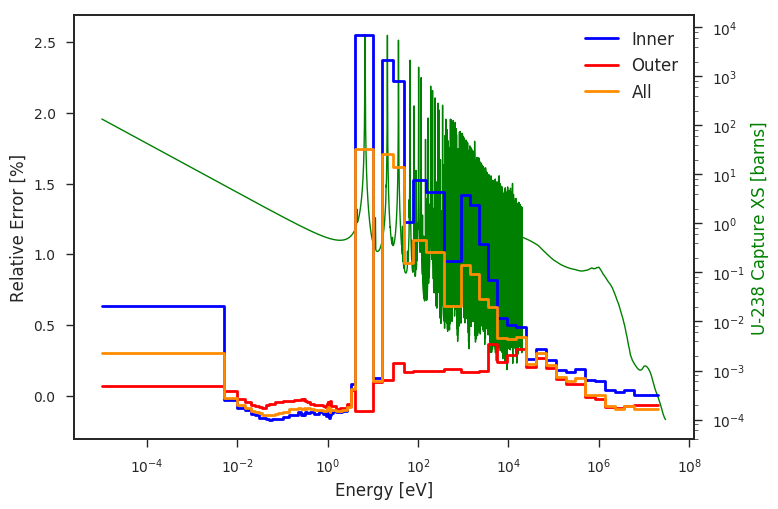
\includegraphics[width=\linewidth]{figures/rel-err-inner-outer}
\caption{The energy-dependent relative error of the OpenMOC scalar flux with respect to the reference OpenMC flux for the innermost, outermost and all FSRs.}
\label{fig:rel-err-energy}
\end{figure}

\begin{figure}[H]
\centering
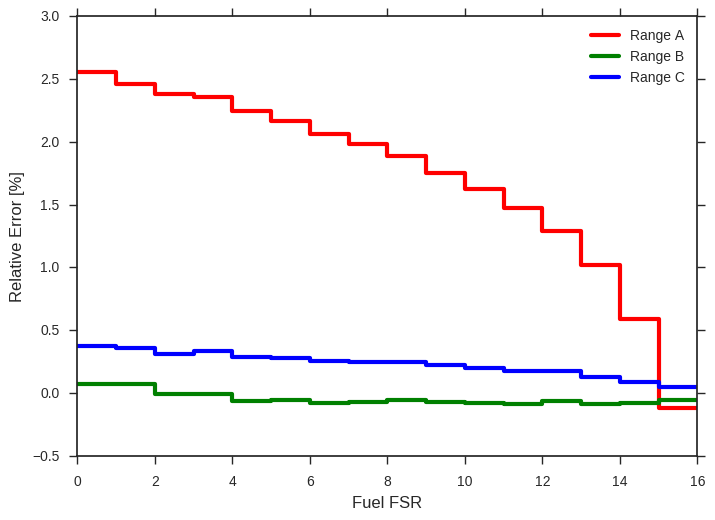
\includegraphics[width=0.8\linewidth]{figures/rel-err-fuel-fsrs}
\caption{The spatially-varying relative error of the OpenMOC scalar flux with respect to the reference OpenMC flux in energy Ranges A, B, and C.}
\label{fig:rel-err-space}
\end{figure}